\documentclass{article}
\usepackage{graphicx} % Required for inserting images
\usepackage{varwidth}
\usepackage{xcolor}
\usepackage{listings}

\definecolor{codegreen}{rgb}{0,0.6,0}
\definecolor{codegray}{rgb}{0.5,0.5,0.5}
\definecolor{codepurple}{rgb}{0.58,0,0.82}
\definecolor{backcolour}{rgb}{0.95,0.95,0.92}

\lstdefinestyle{CStyle}{
	language=C++,
	backgroundcolor=\color{backcolour},   
	commentstyle=\color{codegreen},
	keywordstyle=\color{magenta},
	numberstyle=\tiny\color{codegray},
	stringstyle=\color{codepurple},
	basicstyle=\ttfamily\footnotesize,
	breakatwhitespace=false,         
	breaklines=true,                 
	keepspaces=true,                 
	numbers=left,       
	numbersep=5pt,                  
	showspaces=false,                
	showstringspaces=false,
	showtabs=false,                  
	tabsize=2,
}
\lstset{style=CStyle}

\title{Lab 2 Report \\ \large EEL4742C - 00446}
\author{Yousef Awad}
\date{September 2025}
\setcounter{secnumdepth}{0}

\begin{document}

\maketitle
\tableofcontents
\newpage

\section{Introduction}
Lab 2 introduces us to the 2 push buttons (not counting the reset one) on the MSP430 boards we are using. Alongside this we also found out that the buttons are wired in an active low configuration and therefore gets us used to configuring the built-in pull-up resistors that are on the microcontroller. We also learn how to detect when the buttons are pressed, released, and held all while utilizing our knowledge from Lab 1.

\section{2.1) Turning on the LED with the Button}
This part is the one that specifically shows us how the button works and how the registers are configured. Specifically we set the direction register to be input, and enable the pull-up resistor needed for the first button. After this we use an if statement to check the state of the button and turn on LED while the button is pressed.
\begin{lstlisting}
#include <msp430.h>

#define BUT1 BIT1
#define BUT2 BIT2

#define RLED BIT0
#define GLED BIT7

int main(void)
{
	WDTCTL = WDTPW | WDTHOLD; // stop watchdog timer
	PM5CTL0 &= ~LOCKLPM5;

  // Outputs are red led and green led
  P1DIR |= RLED;
  // setting the leds off by defau;t
	P1OUT &= ~RLED;

  P1DIR &= ~BUT1; // INPUT FOR BUTTON 1
  P1REN |= BUT1; // ENABLING P1REN
  P1OUT |= BUT1; // ENABLING P1OUT FOR PULLUP


  for (;;)
  {
    if ((P1IN & BUT1) == 0)
    {
      P1OUT |= RLED;
    }
    else
    {
      P1OUT &= ~RLED;
    }  
	}
}
\end{lstlisting}
As well as here is the schematic of the buttons proper:
\newline
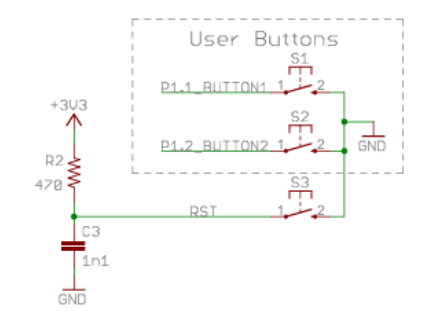
\includegraphics[width=1\textwidth]{pictures/2_1.png}
Specifically, with regards to the schematic, the button is designed to be active-low, or that it actually passes current to Grond when its pressed. It needs a pull up resistor so that there can be 2 differing voltage levels/states to measure.

\section{2.2) Using Two Push Buttons}
This part wants us to just modify the above code and have it include the second button and making it so that when pressing it, it enables the green led, all the while keeping the same functionality from 2.1. The code for it is below.
\begin{lstlisting}
#include <msp430.h>

#define BUT1 BIT1
#define BUT2 BIT2

#define RLED BIT0
#define GLED BIT7

int main(void)
{
  WDTCTL = WDTPW | WDTHOLD; // stop watchdog timer
  PM5CTL0 &= ~LOCKLPM5;

  // Outputs are red led and green led
  P1DIR |= RLED;
  P9DIR |= GLED;
  // setting the leds off by defau;t
  P1OUT &= ~RLED;
  P9OUT &= ~GLED;

  P1DIR &= ~(BUT1 | BUT2); // INPUT FOR BUTTON 1
  P1REN |= (BUT1 | BUT2); // ENABLING P1REN
  P1OUT |= (BUT1 | BUT2); // ENABLING P1OUT FOR PULLUP

  for (;;)
  {
		if ((!(P1IN & BUT1) && !(P1IN & BUT2)))
		{
			P1OUT |= RLED;
			P9OUT |= GLED;
		}
		else if ((P1IN & BUT1) == 0)
		{
			P1OUT |= RLED;
			P9OUT &= ~GLED;
		}
		else if ((P1IN & BUT2) == 0)
		{
			P9OUT |= GLED;
			P1OUT &= ~RLED;
		}
		else
		{
			P1OUT &= ~RLED;
			P9OUT &= ~GLED;
		}
  }
}
\end{lstlisting}

\section{2.3) Electric Generator Load Control (v1)}
For part 3 we were told to make the control for a hypothetical machine that has 2 outputs/machines to run/signal. These 2 outputs, however, \textbf{cannot} be run at the same, else it puts too much stress on the system and will, from my imagination, explode. To this end, when one button is pressed (and therefore one machine is powered), no matter if we press the other button, the other machine will not recieve power and will remain like this only until the original button is unpressed. To that end, here is the code below...
\begin{lstlisting}
#include <msp430.h>

#define BUT1 BIT1
#define BUT2 BIT2

#define RLED BIT0
#define GLED BIT7

int main(void)
{
  WDTCTL = WDTPW | WDTHOLD; // stop watchdog timer
  PM5CTL0 &= ~LOCKLPM5;

  // Outputs are red led and green led
  P1DIR |= RLED;
  P9DIR |= GLED;
  // setting the leds off by defau;t
  P1OUT &= ~RLED;
  P9OUT &= ~GLED;

  P1DIR &= ~(BUT1 | BUT2); // INPUT FOR BUTTON 1
  P1REN |= (BUT1 | BUT2); // ENABLING P1REN
  P1OUT |= (BUT1 | BUT2); // ENABLING P1OUT FOR PULLUP
  
  for (;;)
  {
		if (!(P1IN & BUT1) && !(P1IN & BUT2))
		{
			continue;
		}

		if (!(P1IN & BUT1))
		{
			P1OUT |= RLED;
			P9OUT &= ~GLED;
		}
		else if (!(P1IN & BUT2))
		{
			P9OUT |= GLED;
			P1OUT &= ~RLED;
		}
		else
		{
			P1OUT &= ~RLED;
			P9OUT &= ~GLED;
		}
  }
}
\end{lstlisting}

\section{2.4) Electric Generator Load Control (v2)}
For this part, we were told that the previous design had too loose of a policy on simultaneous power requests (I guess someone put in a faulty reciever or smoething....). To that end, we need to make it so that if both buttons are pressed then the machines both lose power until only one button is released.
\begin{lstlisting}
#include <msp430.h>

#define BUT1 BIT1
#define BUT2 BIT2

#define RLED BIT0
#define GLED BIT7

int main(void)
{
  WDTCTL = WDTPW | WDTHOLD; // stop watchdog timer
  PM5CTL0 &= ~LOCKLPM5;

  // Outputs are red led and green led
  P1DIR |= RLED;
  P9DIR |= GLED;
  // setting the leds off by defau;t
  P1OUT &= ~RLED;
  P9OUT &= ~GLED;

  P1DIR &= ~(BUT1 | BUT2); // INPUT FOR BUTTON 1
  P1REN |= (BUT1 | BUT2); // ENABLING P1REN
  P1OUT |= (BUT1 | BUT2); // ENABLING P1OUT FOR PULLUP

  for (;;)
  {
		if (!(P1IN & BUT1) && !(P1IN & BUT2))
		{
			P1OUT &= ~RLED;
			P9OUT &= ~GLED;
			while (!(P1IN & BUT1) || !(P1IN & BUT2))
			{
				P1OUT &= ~RLED;
				P9OUT &= ~GLED;
			}
		}
		if (!(P1IN & BUT1))
		{
			P1OUT |= RLED;
			P9OUT &= ~GLED;
		}
		else if (!(P1IN & BUT2))
		{
			P9OUT |= GLED;
			P1OUT &= ~RLED;
		}
		else
		{
			P1OUT &= ~RLED;
			P9OUT &= ~GLED;
		}
  }
}
\end{lstlisting}

\section{Student Q and A}
\subsection{1) When a pin is configured as input, P1IN is used for data, which leaves P1OUT available for other use? In such case, what is P1OUT used for?}
In such a case that P1IN is configured for data, and therefore the direction of the pin is that of INPUT, it would leave P1OUT to be used to control the resistor configuration to either be pull-up or pull-down.

\subsection{2) A programmer wrote this line of code to check if bit 3 is equal to 1: $if((Data\ \&\ BIT3)==1)$. Explain why this if-statement is incorrect.}
This statement isn't correct due to it checking for it being 1 meaning that it is only checking if BIT1 is enabled (of which will never be true due the AND operation with BIT3 (or the decimal number 4)).

\subsection{3) Evaluate this lab’s codes regarding power-efficiency if the device is battery operated. Is reading the button via polling power efficient?}
This lab's code is objectively pretty power inefficient if it was applied via battery power. The reading by polling is inherently inefficient due to it always trying to gather input at all times. A better way would be using the interrupts we learned about in class and only actually doing things when a change in state is found.

\section{Conclusion}
This lab was quite fun to do. It helped a lot with bit masking and solidifying it as well as actually explained what the active-low setup even means. Alongside this, working with the buttons made it so that I now know how to track their input states on the MSP430 as well as having to relate it to the schematic on \textit{literally} declaring which resistor to use was very very interesting to learn. Thank you so much for a very cool lab!!

\end{document}
